\section{Introduction}

In this chapter, we perform simulations to gauge the effectiveness of the DSD metric in improving the prediction of labels on data for scale-free networks [CITE], Watts-Strogatz small-world networks [CITE], and some networks we constructed with hypotheses of how the DSD metric should affect classification on them. We compare the DSD metric with the shortest-path distance metric, which is used in some modern approaches of label prediction, such as k-nearest neighbor classifiers [CITE] and laplacian eigenmaps [CITE]. Although several methods for measuring distance or similarity among vertices in a network use the shortest-path distance in the network, the DSD metric is designed to capture distinctions in similarity not captured by the shortest-path distance alone. Thus, we compare effectiveness of the DSD metric and the shortest-path distance metric. We expect the shortest path distance metric to be less effective than the DSD metric for networks with high clustering coefficients or networks with a small diameter, such as small-world networks. Any vertex in such a network is close to any other node in the network, making the shortest-path distance of any two nodes close. We also expect the DSD metric to be more effective on networks with hub vertices, since these vertices tend to make the network highly connected with a small diameter.

In the same way, we compare the DSD metric with centrality and node influence measures, which are designed to capture the influence of vertices in a graph. Centrality identifies the most important vertices in a graph using various methods such as network flows and walks on the graph [CITE]. Various centrality indices are defined using different properties of vertices that capture different distinctions in similarity than the DSD metric. We study several types of centralities including degree centrality, eigenvector centrality, and dissimilarity based centrality measures. These notions of centrality are more related to the DSD metric than the shortest-paths metric, so we expect that they will be similarly effective in predicting labels.

We hope to reveal properties of graphs that allow the DSD metric to be more effective at classification.

\section{Complete Graph with Hubs}
In this section, we construct of a family of graphs with an intuitive initial labeling of vertices and run simulations on this graph to determine the difference in effectiveness between the DSD metric and the shortest path metric on this family of graphs. We expect the DSD metric to be more effective than the shortest-path distance metric on this family of graphs due to the introduction of hub vertices and the small diameter of the graph.

\subsection{Graph Construction}
We construct a graph starting with two complete graphs of size $n$ and $m$ (referred to as left component and right component, respectively). A complete graph is defined as a graph in which every pair of vertices is connected by an edge. All nodes in the left component were labeled "red", and all nodes in the right component were labeled "blue". We call the disjoint union of the left and right components as the graph $G = (V,E)$, with vertex set $V$ and edge set $E$. We consider all unique pairs of vertices $u,v$ $\epsilon$ $V$ (where $u \neq v$ and $(u,v)=(v,u)$). With a probability $p$, for each pair of vertices, if the edge $(u,v)$ exists, we remove that edge from $E$, and if the edge $(u,v)$ does not exist, we add that edge to $E$. This essentially takes the entries of the adjacency matrix (excluding the diagonal) and replaces $0$'s with $1$'s and $1$'s with $0$'s with a probability $p$. We then create hub vertices and add an edge from every vertex in $V$ (including the recently added hub vertices) to the hub vertices with a high probability $q$. Lastly, we take the largest connected component of this graph and set it as our graph $G$.

\begin{figure}[h!]
\centering
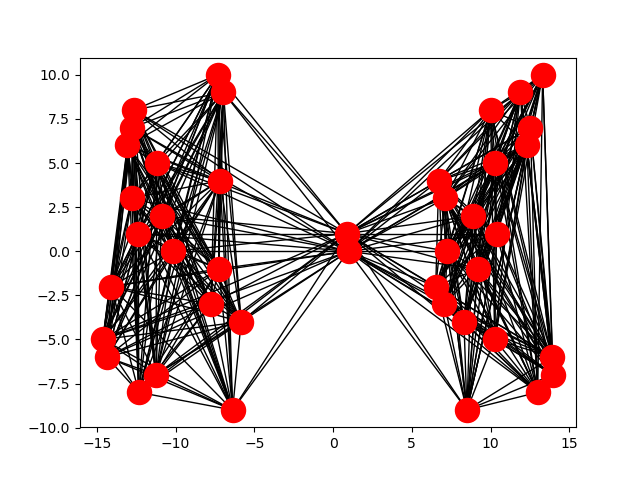
\includegraphics[width=0.6\textwidth]{Sim_Complete_Graph_With_Hubs_p0.png}
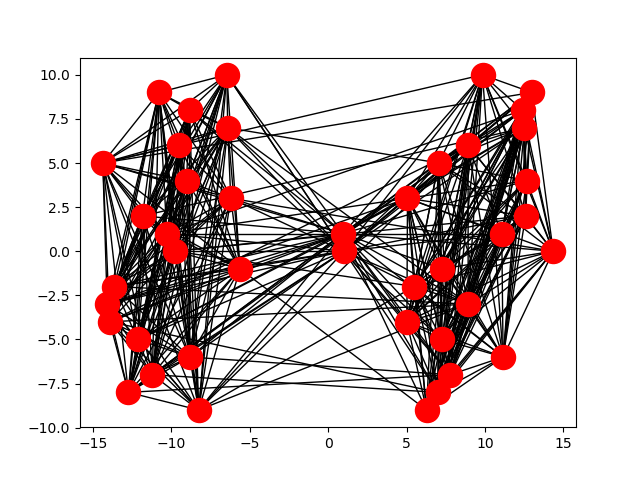
\includegraphics[width=0.6\textwidth]{Sim_Complete_Graph_With_Hubs_p05.png}
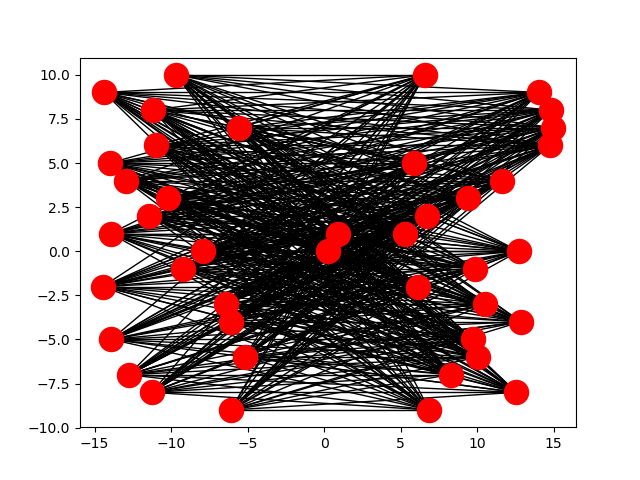
\includegraphics[width=0.6\textwidth]{Sim_Complete_Graph_With_Hubs_p1.png}
\caption{A visualization of the graph constructed from the previous section. Each component has 20 vertices and there are two hub nodes. The probability of adding an edge to a hub node was set to $0.8$, and the probability of flipping an edge was set to $0$, $0.5$, and $1$, respectively.}
\label{fig:complete_graph_with_hubs_1}
\end{figure}

\subsection{Data Collection}
To collect data, we constructed a graph using the method mentioned above, and found the DSD distances for the graph. We censored labels of vertices in the graph with a $0.3$ probability, then tried to predict the censored labels using a weighted majority vote algorithm. All vertices were considered when voting for the label of a single vertex, and each vertex was weighted by the inverse of its degree. The label with the highest voting value was set as the predicted label for the vertex. We recorded the total number of censored vertices, and the number of correctly predicted vertices, calculating the percent of correctly predicted labels using the ratio of these values.

Our results were compared to the shortest path distance and the random labeling straw man.


% Add a table of data

\subsection{Analysis}
\noindent
Compare shortest paths distances data with DSD data. Analyze results.

